\documentclass[]{article}
\usepackage[utf8]{inputenc}
\usepackage{tikz}
\usepackage{hyperref}
\usepackage{titling}
\usepackage{enumitem}
\usepackage{titlesec}
\usepackage[margin=1.5in]{geometry}

%opening
\title{Draw.3D}
\author{Ida Hönigmann \and Manuel Eiwen \and Mathias Eitler}

\begin{document}

\maketitle

\section*{Idee}
Benutzer können durch Bewegung ihrer Handys in einer 3D Umgebung ,,zeichnen''.

\section*{Anwendung}
Die Benutzer verbinden sich mit einem Server. Auf dem Server wird in einem Browser eine 3D Umgebung angezeigt. Durch Änderung der Orientierung (rotieren) des Handys kann man seine Position in der 3D Umgebung verändern und es wird eine Linie zu der neuen Position / eine Kugel auf der neuen Position gezeichnet.
Es soll möglich sein, dass mehrere Personen mit ihren Handys gleichzeitig in der gleichen 3D Umgebung zeichnen.

\section*{Themengebiete}
Im Rahmen des Projekts sollen die folgenden Themengebiete näher erforscht werden:
\begin{itemize}[noitemsep,topsep=4pt]
	\item Orientierungsdaten von Handys mittels Javascript erhalten
	\item Kommunikation der Orientierungsdaten an einen Server mittels Websockets
	\item Umrechnen von Orientierungsdaten in Positions-Koordinaten
	\item Darstellen von 3D-Grafiken in Browsern
\end{itemize}

\section*{Implementierung}
Die Verbindung zwischen den Handys und dem Server soll mittels Websockets implementiert werden. Nachdem sich ein Handy verbunden hat fragt das Programm (mehr oder weniger) durchgehend die derzeitige Orientierung des Handys ab.\footnote{ähnlich diesem \href{https://developer.mozilla.org/en-US/docs/Web/API/Detecting\_device\_orientation}{Beispiel}} Da diese Daten keine Information zur Position geben werden sie (durch eine künstlich hinzugefügte) Beschleunigung ergänzt und zu Positionsdaten (x-, y- und z-Koordinaten) umgewandelt.

\subsection*{Darstellung auf Server}
Diese Positionsdaten werden dann zum Server geschickt, der diese mittels einer 3D Grafik Library\footnote{mögliche Libraries können \href{https://1stwebdesigner.com/3d-javascript-libraries/}{hier} gefunden werden} für JavaScript darstellt. Ob die Position in Form einer Linie zur aktuellen Position oder einfach einer Kugel auf der aktuellen Position dargestellt wird (oder ob beides möglich sein soll) wird noch im Rahmen des Projekts entschlossen.

Auf jeden Fall muss jeder Client eine Farbe auswählen, in dieser die Kugel bzw. die Linie auf dem Server dargestellt wird.

\subsection*{Darstellung auf Clients}
Um die Bedienung verständlicher zu machen wird auf jedem Client ein Kreis angezeigt, der mit Veränderung der Neigung des Clients seine Position verändert. Außerdem sollen auch die Neigungen aller anderen Clients als Kreis angezeigt werden, wobei der eigene Kreis weiß ist und die Restlichen in der von den Clients ausgewählten Farbe. Des weiteren wird die eigene Farbe als Hintergrundfarbe verwendet.

\section*{Kommunikation}
Die ausgerechneten Positionsdaten aller Handys werden alle x Millisekunden an den Server geschickt. Dieser Verarbeitet diese sobald er sie erhält. Eine beispielhafte Kommunikation zwischen drei Handys und einem Server kann in Abbildung~\ref{fig:kommunikationsdiagramm} gefunden werden.

\begin{figure}[!h]
	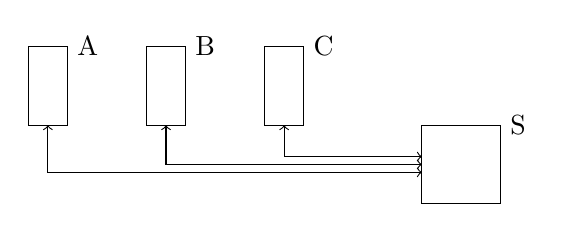
\begin{tikzpicture}
	\draw (3,1) rectangle (3.5,2) node (C) [right] {C};
	\draw (1.5,1) rectangle (2,2) node (B) [right] {B};
	\draw (0,1) rectangle (0.5,2) node (A) [right] {A};
	
	\draw (5,0) rectangle (6,1) node (S) [right] {S};
	
	\draw [<->] (3.25,1) -- (3.25,0.6) -- (5,0.6);
	\draw [<->] (1.75,1) -- (1.75,0.5) -- (5,0.5);
	\draw [<->] (0.25,1) -- (0.25,0.4) -- (5,0.4);
	\end{tikzpicture}
	\caption{Drei Handys (gekennzeichnet mit A, B und C) schicken ihre Orientierungsdaten an einen Server (gekennzeichnet mit S), der diese dann grafisch darstellt.}
	\label{fig:kommunikationsdiagramm}
\end{figure}

Die Daten, die an den Server geschickt werden müssen sind:
\begin{verbatim}
{
id: <eindeutige Identifikation des Clients>,
color: <Farbe des Clients>,
alpha: <Rotation entlang der z-Achse>,
beta: <Rotation entlang der x-Achse>,
gamma: <Rotation entlang der y-Achse>
}
\end{verbatim}

\end{document}
